
\documentclass[letterpaper,12pt]{article}
\usepackage{tabularx} % extra features for tabular environment
\usepackage{amsmath}  % improve math presentation
\usepackage{float}
\usepackage{pdfpages}

\usepackage{multicol}
\usepackage{graphicx} % takes care of graphic including machinery
\graphicspath{ {./figures/} }
%\usepackage[margin=1in,letterpaper]{geometry} % decreases margins
%\usepackage{cite} % takes care of citations
\usepackage[final]{hyperref} % adds hyper links inside the generated pdf file
\hypersetup{
	colorlinks=true,       % false: boxed links; true: colored links
	linkcolor=blue,        % color of internal links
	citecolor=blue,        % color of links to bibliography
	filecolor=magenta,     % color of file links
	urlcolor =blue         
}
\usepackage[margin = 1in,headsep=0.5cm,headheight=2cm,letterpaper]{geometry} 

\usepackage{fancyhdr}
\pagestyle{fancy}
\lhead{Student 1 : Ahmet Akman 2442366 \\ Student 2: Yusuf Toprak Yıldıran 2444149 \\ Assistant: Onur Selim Kılıç}
\rhead{Date: \today \\ Group: Wednesday Morning - 5} 
%\cfoot{center of the footer!}
\renewcommand{\headrulewidth}{0.1pt}



\begin{document}
\thispagestyle{empty}

\title{Spring 2022 EE214 Experiment 7  \protect\\ Active RC Filters}
\author{Ahmet Akman 2442366 \protect\\ Yusuf Toprak Yıldıran 2444149 \protect\\ Assistant: Onur Selim Kılıç}
\date{\today}
\maketitle
\tableofcontents
%\begin{abstract}
%abstract
%\end{abstract}
\section{Introduction}

\section{Experimental Results and Discussion}
The results of the experiment are discussed in the following steps.
\subsection{Step 1}

In this part, circuit in figure 1 is set with an input sine wave of 1V peak. Then, max output voltage is found and recordeed as center frequency by manually changing the frequency. Afterwards, half power frequency which is equal to 0.7 times of the center frequency is found by trying the frequencies and these values are recorded in table 1.   
\begin{figure}[H]
    \centering
    \includegraphics[width = 0.75\textwidth]{{1_1.png}}
    \caption{Circuit for step 1}
\end{figure}


\begin{table}[H]
    \begin{center}
        \caption{Measurements}
        \vspace{2mm}
        \begin{tabular}{||c | c | c | c | c | c||} 
            \hline
            \(w_c\) & \(H(w_c)\) & \(|H(w_c)|\) & \(|H(w_0)|\) & \(H(w_0)\) \\ [0.5ex] 
            \hline\hline
            a & a & a & a & a \\ 
        
            \hline
        \end{tabular}
    \end{center}
    \end{table}

Afterwards, frequency and phase response of the cicuit are obtained using computer BenchVue test flow with DC sweep from \(\frac{f_c}{5}\) to \(5f_c\) with the steps \(\frac{f_c}{10}\).

After making necessary test flow settings and run the test, magnitude and frequency responses of the circuit are obtained. Then, datas are exported to MATLAB and \(w_0\) ,\(w_1\), and \(w_2\) are determined from magnitude response plot and showed as in Figure 2.  

\begin{figure}[H]
    \centering
    \includegraphics[width = 0.75\textwidth]{{1_1.png}}
    \caption{Magnitude and Phase response of circuit 1}
\end{figure}

\subsection{Step 2}


\section{Conclusion}


\section*{Appendix A}
\begin{itemize}
    \item PreLab Preparation 2 hours
    \item Experimental Work 2  hours
    \item Report Writing 9 hours
\end{itemize}

\end{document}

%%%%%%%%%%%%%%%%%%%%%%   EXAMPLE TABLE   %%%%%%%%%%%%%%%%%%%%%%%%%%%%%%%%
\begin{table}[H]
\begin{center}
    \caption{Resistance reading by color code convention.}
    \vspace{2mm}
    \begin{tabular}{||c | c | c||} 
        \hline
        Color Order & Value & Tolerance \\ [0.5ex] 
        \hline\hline
        Brown / Black / Red / Gold & 1k\( \Omega \) & \( \% \) 5  \\ 
        \hline
        Yellow / Violet / Red / Gold & 4.7k\( \Omega \) & \( \% \) 5   \\
        \hline
        Brown / Grey / Orange / Gold & 18k\( \Omega \) & \( \% \) 5  \\ [1ex] 
        \hline
    \end{tabular}
\end{center}
\end{table}


%%%%%%%%%%%%%%%%%%%%%%   EXAMPLE IMAGE   %%%%%%%%%%%%%%%%%%%%%%%%%%%%%%%%
\begin{figure}[H]
\centering
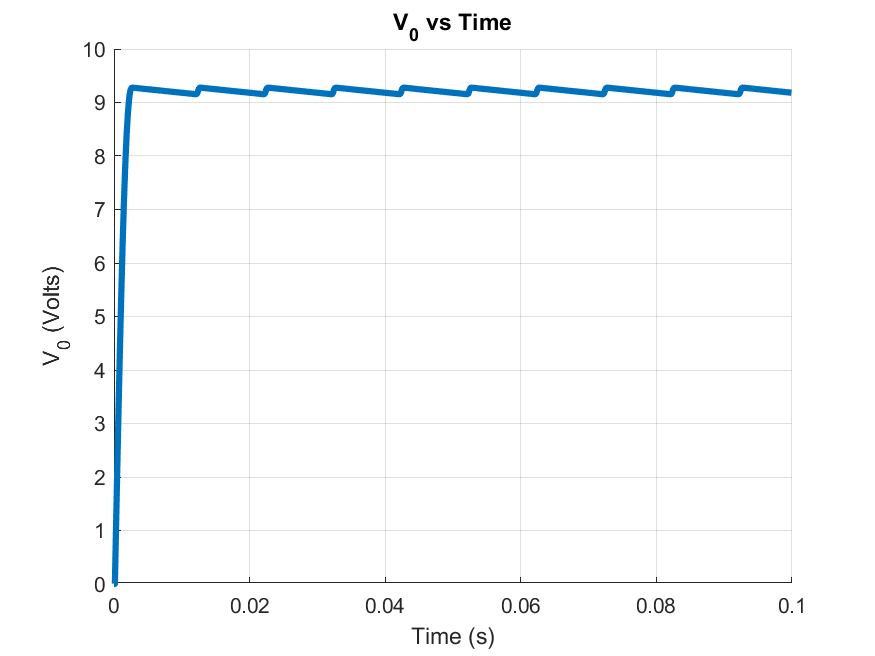
\includegraphics[width = 0.75\textwidth]{5.png}
\caption{Circuit schematic for the step 5}
\end{figure} 

%%%%%%%%%%%%%%%%%%%%%%   EXAMPLE IMAGE FROM PDF   %%%%%%%%%%%%%%%%%%%%%%%%%%%%%%%%
\begin{figure}[H] \centering{
	\includegraphics[scale=0.25]{2a_plot.pdf}}
	\caption{Experiment 2}
\end{figure}
